
\section{Methodology}
\label{sec:methodology}
In order to \LK{study} the stability of applications run on a superconducting transmon device we selected the Boeblingen IBM Quantum hardware platform, which is a 20-qubit quantum computing hardware platform with a qubit layout as shown in Fig.~\ref{fig:Boeblingen_layout}. 
\begin{figure}[htpb]
    \centering
    % 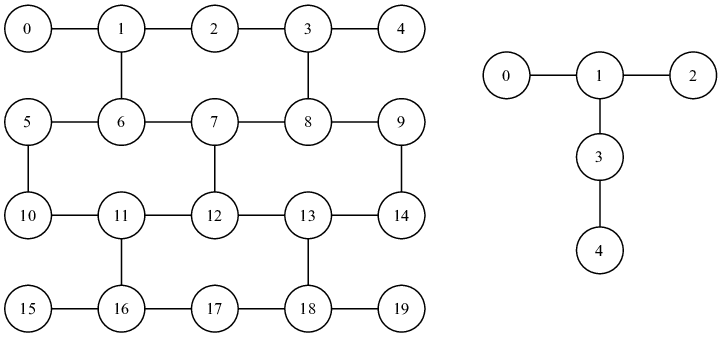
\includegraphics[width=\columnwidth,
    % clip=true,trim=0 0 280 0]{boeblingen.png}
    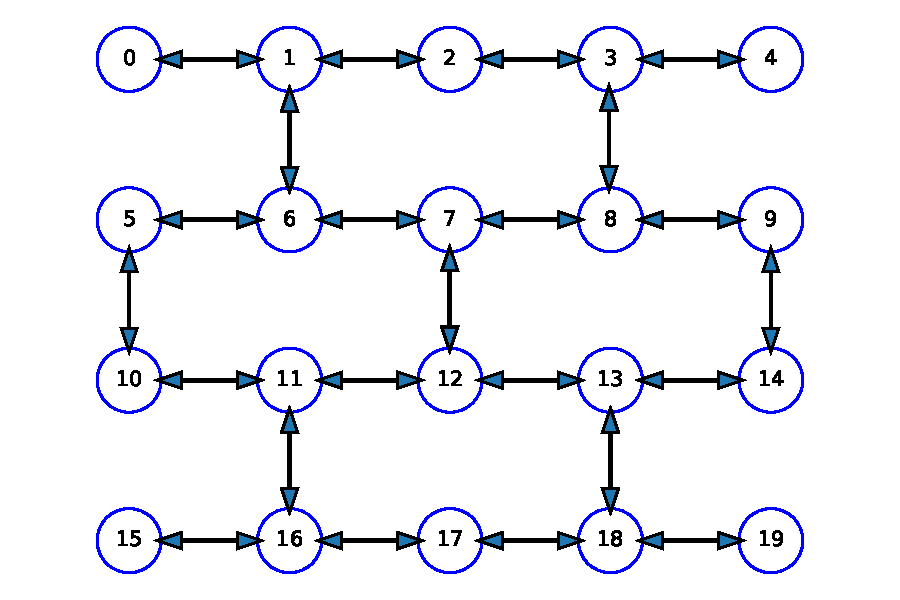
\includegraphics[scale=0.4]{QubitsBoeblingen.pdf}
    \caption{Qubit layout for \emph{ibmq\textunderscore  boeblingen}.    }
    \label{fig:Boeblingen_layout}
\end{figure}

The Transverse Ising model Hamiltonian discussed in Sec \ref{sec:model} and the
quantum circuit diagram of the TIM (Fig.~\ref{fig:IsingTrotterCircs}) represented the application used to test the stability of the IBMQ Boeblingen processor. These two quantum circuits are equivalent circuit combinations because the gates representing the different terms in the Hamiltonian commute with each other. Both of these quantum circuits result in time evolution \LK{for a time $\delta t$} of a state with $\mathcal{U}=e^{-iH_{\text{OBC}}\delta t}$ using Trotterization where $\delta t$ is the time interval for one Trotter step. 


\begin{figure*}[!tb]
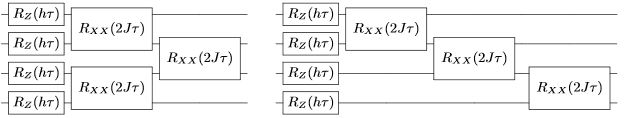
\includegraphics[width=\textwidth]{Circuits1.JPG}
%\[ {\Qcircuit @C=0.5em @R=0.5em {
%     \lstick{} & \gate{R_Z(h \tau)} & \multigate{1}{R_{XX}(2 J \tau)} &\qw&\qw  & & & &\\ 
%     \lstick{} & \gate{R_Z(h \tau)}  & \ghost{R_{XX}(2 J \tau)} & \multigate{1}{R_{XX}(2 J \tau)}&\qw & & & &\\
%     \lstick{} &  \gate{R_Z(h \tau)} & \multigate{1}{R_{XX}(2 J \tau)}&\ghost{R_{XX}(2 J \tau)}&\qw & & & & \\
%     \lstick{} &  \gate{R_Z(h \tau)} & \ghost{R_{XX}(2 J \tau)} &\qw&\qw& & & &}}
%    { \Qcircuit @C=0.5em @R=0.5em {
%     \lstick{} & \gate{R_Z(h \tau)} & \multigate{1}{R_{XX}(2 J \tau)} &\qw&\qw &\qw & \qw\\ 
%     \lstick{} & \gate{R_Z(h \tau)}  & \ghost{R_{XX}(2 J \tau)} & \multigate{1}{R_{XX}(2 J \tau)}&\qw&\qw&\qw \\
%     \lstick{} &  \gate{R_Z(h \tau)} & \qw&\ghost{R_{XX}(2 J \tau)}&\qw & \multigate{1}{R_{XX}(2 J \tau)} & \qw \\
%     \lstick{} &  \gate{R_Z(h \tau)} & \qw &\qw&\qw&\ghost{R_{XX}(2 J \tau)} & \qw}\]
\caption{The quantum circuit for one Trotter step of the time evolution with the open boundary condition Ising model Hamiltonian. We define the quantum circuit in left (right) panel as Circuit 1 (Circuit 2).}
\label{fig:IsingTrotterCircs}
\end{figure*}


Because the two-qubit gates in quantum circuits are a major source of the errors generated in a quantum computer, this project focused on studying the behavior of these gates under various conditions. From the circuit diagram, it is seen that there were three pairs of two-qubit CNOT gates that are needed to construct this circuit. The CNOT gates that exist in two circuit configurations that were labelled as Circuit 1 and Circuit 2 can be seen in Fig.~\ref{fig:hardcycles}.

\begin{figure}[htpb]
    % \centering
    % \includegraphics[width=2.2\columnwidth]{final_plot.pdf}
    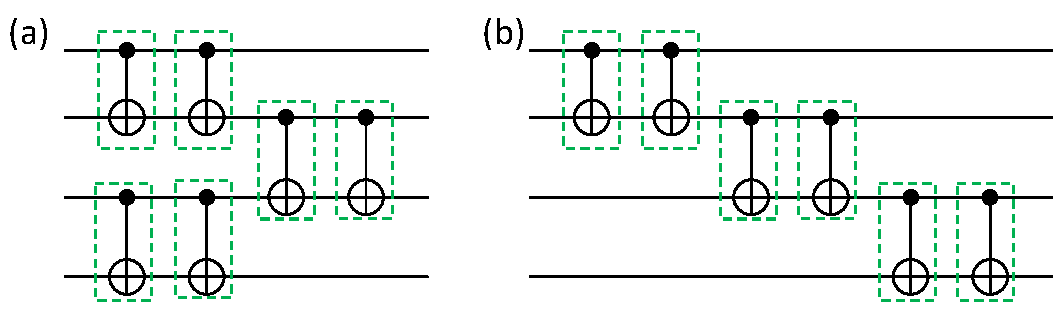
\includegraphics[scale=0.50]{hardcyclesCirc1Circ2.pdf}
    \caption{The CNOT hard cycles used at each Trotter step for circuit 1 ({\bf{(a)}}) and circuit 2 ({\bf{(b)}}) to calculate QCAP$_{\text{CB}}$ bound from cycle benchmarking are shown in dashed boxes.}
    \label{fig:hardcycles}
\end{figure}

% \textbf{need pdf of the two circuit layouts showing the CNOT gates}.
(In our experiments, we chose one Trotter step as $\delta t=10$.) \LK{What is $\delta t$ in units of the physics constants?} The only difference in these two circuits is that circuit 2 has a deeper number of steps \LK{What does this mean?} compared to circuit 1 when being evaluated. Both circuit 1 and circuit 2 formed the gates of interest in a \LK{recent} cycle benchmarking computation \cite{CB-Nat-Comm-2019}.  A detailed discussion of cycle benchmarking can be found in the Appendix~\ref{sec:cyclebenchmarking}. 

The cycle benchmarking procedure used C1 twirling rather than the Pauli twirling so that these computations would complete within the morning and night dedicated time windows. The C1 twirling used random single qubit Cliffords which had the effect of symmetrizing the X, Y and Z noise.  This would ultimately allow for an analysis of the depolarization error, which is one of the simplest of the systematic errors.  

To calculate the process infidelity, $e_F$, contribution of each of the 16 possible combinations of Pauli decay terms, three different C1 sequence circuit lengths (lengths of 2, 10 and 22) were run.  This set of equations were then solved to calculate $e_{F}$, the value of the total probability that an error afflicts the targeted systems during a dressed gate ( 
define dressed gate)

For each of the three different layouts, individual process infidelity calculations were done using different pairs of CNOT gate combinations for each of the three different qubit layouts on IBMQ Boeblingen device.  C1 twirling was done using gate sequence circuit lengths of 2, 10, and 22 random Clifford gates were applied to each of the different pair combinations of CNOTs.  The combination of the CNOT gate being measured and the sequence of random Cliffords is defined as a dressed cycle of the CNOT gates being measured.  The process infidelity of the dressed cycle for that CNOT pair {\color{red}{KYA: why do we say the CNOT pair? CB was done on individual CNOTs.}} was computed based on the calculated values of each of the Pauli decay terms.  The overall process infidelity for each pair of CNOT gates was then compared to the published values of the pairs of CNOT gates in the IBM Quantum backend properties that were measured using randomized benchmarking. For a fair comparison, we converted the published CNOT average gate infidelities to process infidelities using a dimensional factor.  




The team \LK{We} selected three separate groups of qubits on the Boeblingen hardware platform as indicated in Fig.~\ref{fig:Boeblingenlayout} \sout{to run Circuit 1 and Circuit 2 with the cycle benchmarking computation} \KYA{to study the error characterization of TIM Trotterization circuits using CB}.  The qubit group in the upper left hand corner [0, 1, 2, 3] was labelled ``Layout 1", a group of qubits in the center [6, 7, 12, 11] was labelled ``Layout 2", and a third group of qubits in the lower right [16, 17, 18, 19] was labelled ``Layout 3".  

\begin{figure}[htpb]
    \centering
    % 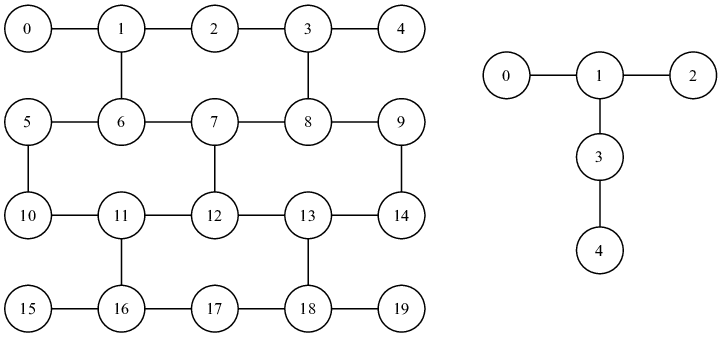
\includegraphics[width=\columnwidth,
    % clip=true,trim=0 0 280 0]{boeblingen.png}
    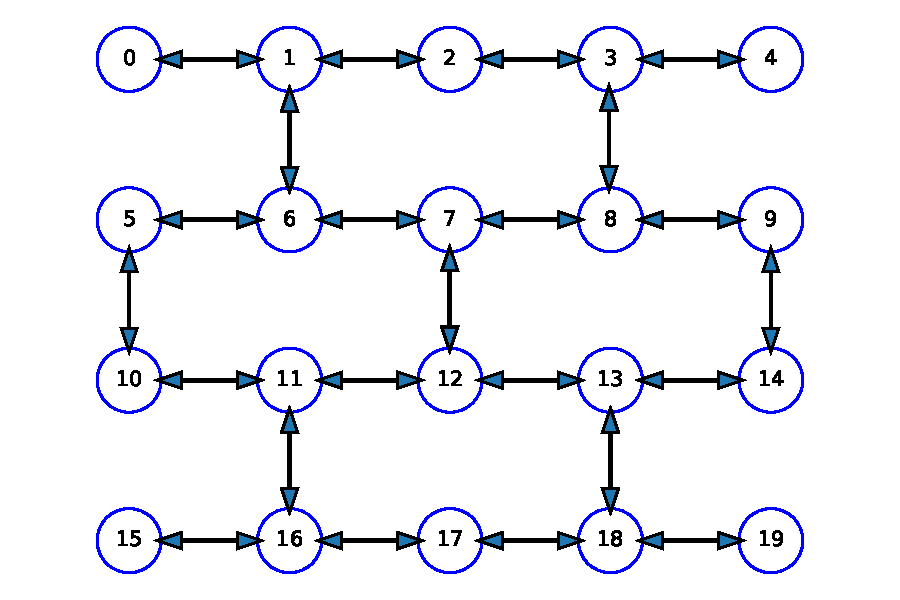
\includegraphics[scale=0.4]{QubitLayoutBoeblingen.pdf}
    \caption{Three different groups of qubits were selected to run the set of cycle benchmarking and TIM computations described in this paper.  Layout 1 refers to qubits [0, 1, 2, 3], Layout 2 refers to qubits [6, 7, 12, 11] and Layout 3 refers to qubits [16, 17, 18, 19]. \LK{This figure is redundant. Consider combining with Fig 3}}
    \label{fig:Boeblingenlayout}
\end{figure}

The set of computations run on Boeblingen consisted of a cycle benchmarking of \KYA{of the CNOT gates applied between qubit pairs in Layout 1, 2, and 3, a calculation of QCAP bound of CNOT hard cycles in} circuit 1 and circuit 2 \KYA{as a function of number of Trotter steps} and a calculation of the transverse Ising model occupation index \KYA{as a function of time}.  The computations were run on Boeblingen hardware in the morning, afternoon and night during eight day consecutive period in January 2021 when the team was able to secure more than 140 hours of dedicated time for access to Boeblingen device.  The team scheduled dedicated reservation time on Boeblingen each day between 4 am to 10 am and again from 3 pm until 11 pm.  By placing Boeblingen into dedicated mode, it guaranteed that the series of computations that our project implemented on Boeblingen to test the stability of the device ran uninterrupted because no other users had access to the machine during those time windows.  

The IBM team at Yorktown Heights agreed to schedule a full re-calibration of Boeblingen device each day beginning at the start of our 4 am morning dedicated time slot. This full re-calibration of the full set of Boeblingen's qubits took approximately 2 hours to complete each morning. The IBM team also agreed to do a separate 2-qubit re-calibration of Boeblingen device each night during our team's dedicated mode time slot starting at 6 pm local time. The 2-qubit night re-calibration took approximately an hour to complete.  Each re-calibration was done when  Boeblingen had no user activity and after each IBM quantum hardware re-calibration was completed the team recorded Boeblingen hardware back-end properties.  

After the morning and night re-calibrations were completed by the IBM team our group ran \KYA{the circuits for CB the CNOT gates in Layout 1, 2, and 3, circuits for calculating the QCAP bound using CB for each CNOT gate in} both the circuit 1 and circuit 2 \sout{computations in cycle benchmarking} and then the calculation of the TIM occupation indexes \KYA{as a function of time} on each of the three different layouts during the dedicated morning, afternoon, and night time windows. Within the cycle benchmarking set of calculation each run included a cycle benchmarking analysis of the CNOT cycles in each layout followed by a separate run for calculation of quantum capacity (QCAP) bound for the Circuit 1 and Circuit 2 CNOT cycles.


\textbf{=====}



When a quantum circuit is run under randomized compiling (RC)~\cite{Wallman2016} since the noise is stochastic, the process infidelity is also a bound on the total variation distance (TVD) between the ideal bitstring distribution of the circuit and the empirical bitstring distribution measured by a quantum device. Therefore, to get a lower bound estimate on the stochastic error for the CNOT cycles of the quantum circuits of TIM Trotterization we performed additional experiments and calculated the Quantum Capacity (QCAP). The QCAP bound is calculated as follows. The QCAP tool available in TrueQ software takes the single circuit as an argument and runs CB circuits for every hard cycle (denotes the multi-qubit operations) in that quantum circuit. The hard cycles of the quantum circuit of interest can be seen in Fig.~\ref{fig:hardcycles}. From these CB runs the process infidelity of each hard cycle is calculated. Even though in the ideal case the CNOT gates in Fig.~\ref{fig:hardcycles} would cancel each other to make an identity, in QCAP calculation process each CNOT cycle is considered separately and CB circuits are concatenated to each of the CNOT gates separately. Finally, under the assumption that the circuits are run under RC and the noise is stochastic, the QCAP bound is calculated from the multiplication of the process fidelity of each hard cycle.  
% This quantity uses a single circuit in the cycle benchmarking procedure to estimate the process fidelity of the entire circuit for each incremental additional circuit added.  
We used the CNOT cycles for each Trotter step of Circuit 1 and Circuit 2 as our circuit argument for calculating the QCAP bound and we calculated and plotted the average process infidelity as a function of number of Trotter steps.
% The average process infidelity versus Trotter step was calculated and plotted for both Circuit 1 and Circuit 2.  
Small values for the average process infidelity versus Trotter step indicate that the circuit will reliably perform over a given Trotter step range.  


Very often CNOTs exhibit coherent/unitary errors due to crosstalk. This QCAP bound can be taken as a reasonable measure of circuit performance on the selected set of qubits if the single qubit backend property error measurements are approximately an order of magnitude smaller than the CNOT errors.  This condition makes it reasonable to approximate the errors from each Trotter step as only having a stochastic contribution.  Assuming there is only a stochastic contribution ensures that the process infidelity is additive and grows linearly in the number of Trotter steps for short depth.




quantum circuits to perform cycle benchmarking and then quantum circuits for calculating the quantum capacity (QCAP) of the Trotterization circuit which





The CB procedure, QCAP calculations and TIM computations were each implemented on three sets of 4 qubits located on different physical sections of the 20-qubit chip (qubits [0, 1, 2, 3] in the upper left, qubits [6, 7, 11, 12] in the center and qubits [16, 17, 18, 19] on the lower right of the IBMQ Boeblingen chip (see Fig.~\ref{fig:BoeblingenCycles})).  In this paper, these qubit configurations are identified as Layout 1, 2 and 3, respectively.  For the cycle benchmarking portion, using the identity and Pauli Z as the set of Cliffords for the cycle benchmarking, the expectation values versus circuit sequence length were measured for circuit lengths of 2, 10 and 22 and plotted. Here, the sequence length refers to the number of times the cycle of interest appears apart from state inversion. The number of random circuits in each sequence length is chosen to be 48 and each of these circuits were run with $N_{\text{shots}}=128$. Using the three different circuit lengths the amplitude and slope of the exponent were calculated for all 16 of the Pauli decay terms, e.g. $IIII$, $ZIII$, $ZZII \dots ZZZZ$.
These calculations were repeated for the exhaustive set of two-qubit pairs within each of the three different layouts and the process infidelity ($e_{F}$) was calculated using cycle benchmarking method for CNOT cycles seen in Fig.~\ref{fig:BoeblingenCycles}. Each row in Fig.~\ref{fig:BoeblingenCycles} corresponds to the CNOT cycles  studied for each qubit layout. There are four cycles studied for each qubit layout and we label each of these unique cycles as cycle 1, cycle 2, cycle 3 and cycle 4, respectively from left to right. For example, on layout 1 measurements included all of the combination of two-qubit pairs ([0, 1 and 2, 3], [0, 1], [1, 2] and [2, 3]).  Similar measurements were taken on the CNOT pairs for Layouts 2 and 3.   Using these measurements the Pauli infidelity terms were measured and each of the error bars were calculated for every one of the 16 Pauli decay terms.  From this information the overall circuit process infidelity and error bar were computed.  Finally, using this information the quantum capacity (QCAP) was calculated versus the step size.  This QCAP bound graph showed how a dressed cycle of a circuit will have a stochastic error model whose process fidelity is estimated directly by cycle benchmarking.  From this graph the performance of the circuit implemented on the set of specific qubits on that specific hardware platform can be measured over time.  


The parameters used for QCAP measurements is as follows. Due to limited access to the dedicated mode on Boeblingen device we use sequence lengths of 4 and 16. The number of random circuits in this case is 30 and each of these circuits were run $N_{\text{shots}}=128$. 


We also computed an estimate to the QCAP bound of CNOT cycles in the TIM Trotterization quantum circuits as a function of the number of Trotter steps calculated from CNOT error rates reported by IBM using randomized benchmarking. To this end, we used the expression for relationship between the average process fidelity and the average gate fidelity as seen in \eqref{eq:err_rate}. For a quantum circuit with $N$ CNOT gates then the QCAP bound calculated using CNOT error rates provided by IBM which are obtained using randomized benchmarking is
\begin{equation}
    \text{QCAP}_{\text{RB}}=1-\prod_{i=1}^N\left(1-\frac{d+1}{d} r_i\right)~.\label{eq:QCAP_RB}
\end{equation}


After the cycle benchmarking computations were finished, the Trotterization of TIM Hamiltonian was run on each of the three different physical qubit layouts using the Circuit 1 gate circuit design so that a direct comparison could be made to previously published results in~\cite{GustafsonIsing}.  The Data Analysis section \ref{sec:data-analysis} then identified specific error mitigation issues based on these procedures.


% \subsection{Cycle Benchmarking Procedure}

% \label{sec:cb}

% {\color{red}{KYA: I think we don't need this section as the procedure is already explained above}}.

% To study the error characterization of the 4 CNOT cycles in three different location of IBMQ Boeblingen quantum processor we used the cycle benchmarking protocol studied in \cite{Erhard2019} and TrueQ software developed by Quantum Benchmark. More information on CB can be found in Appendix~\ref{sec:cyclebenchmarking}. 

% % \subsection{Cycle Benchmarking Procedure?}
% The measured process infidelities ($e_F$) obtained using CB protocol are presented in 


% The cycle benchmarking data was obtained using the following variables. For each cycle of interest we used sequence lengths of 2, 10, and 22, respectively. The sequence length refers to the number of times the cycle of interest appears apart from state inversion. The number of random circuits used in each sequence length is 48. Each of these circuits at each sequence length were run $N_\text{shots}=128$ times. 

% The process infidelity is estimated from the average value of the individual Pauli infidelities.


% % \subsubsection{Process Infidelity Measurements}
% The process infidelity ($e_{F}$) was calculated using cycle benchmarking method for CNOT cycles seen in Fig.~\ref{fig:BoeblingenCycles}. Each row in Fig.~\ref{fig:BoeblingenCycles} corresponds to the CNOT cycles  studied for each qubit layout. There are four cycles studied for each qubit layout and we label each of these unique cycles as cycle 1, cycle 2, cycle 3 and cycle 4, respectively from left to right.

\begin{figure*}[ht!]
    % \centering
    % \includegraphics[width=2.2\columnwidth]{final_plot.pdf}
    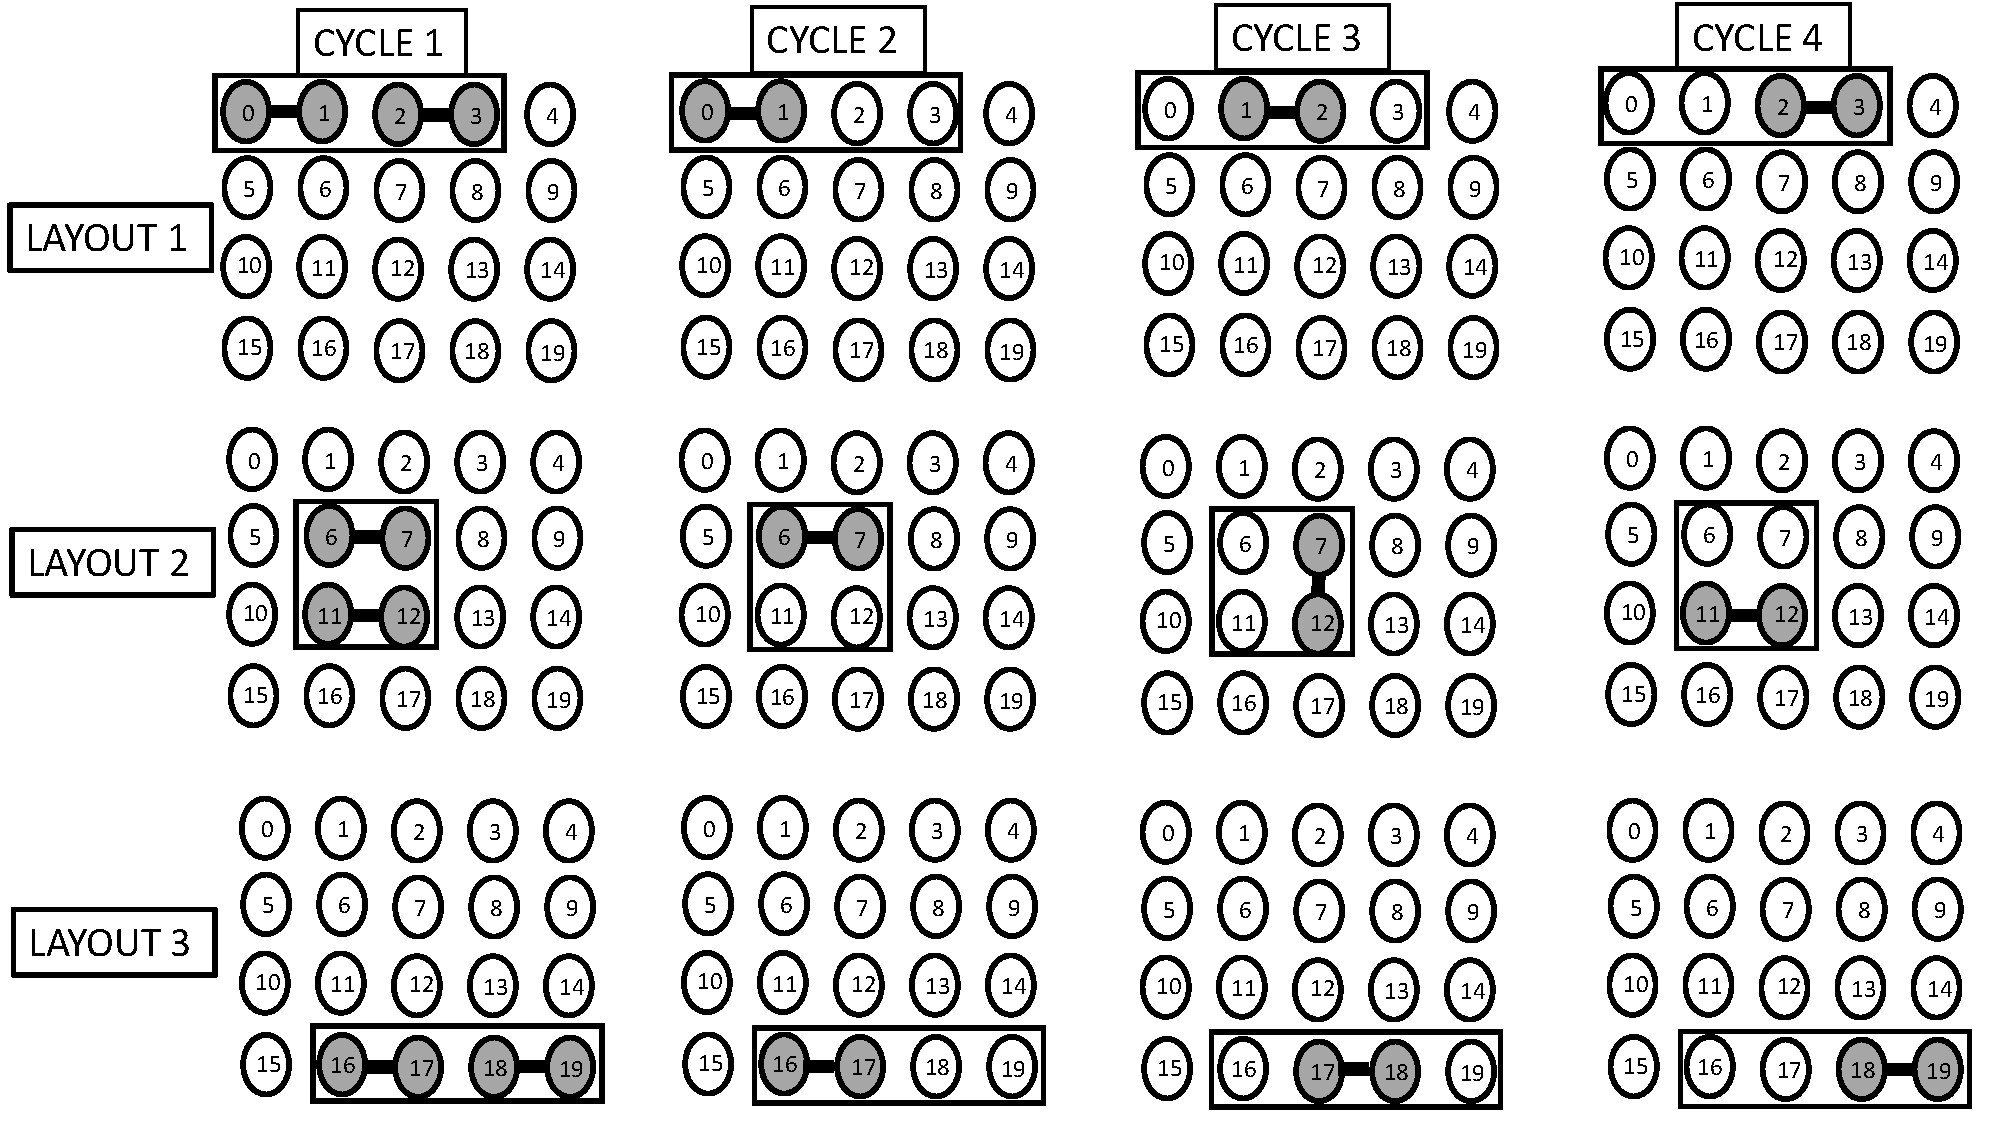
\includegraphics[scale=0.5]{Cycle-Layout.pdf}
    \caption{This figure shows the three different physical qubit layouts selected on Boeblingen and the specific different pairs of qubits paired in each of the four different cycles for each of the three different layouts.  each of the paired CNOTs in each of the four different defined cycles selected  used to calculate the process infidelities for each of the four different defined cycles. CNOT cycles used to calculate the process infidelities on 20-qubit IBM Q Boeblingen device.}
   \label{fig:BoeblingenCycles}
\end{figure*}





% %\begin{figure*}[ht!]
%     % \centering
%     % \includegraphics[width=2.2\columnwidth]{final_plot.pdf}
% %    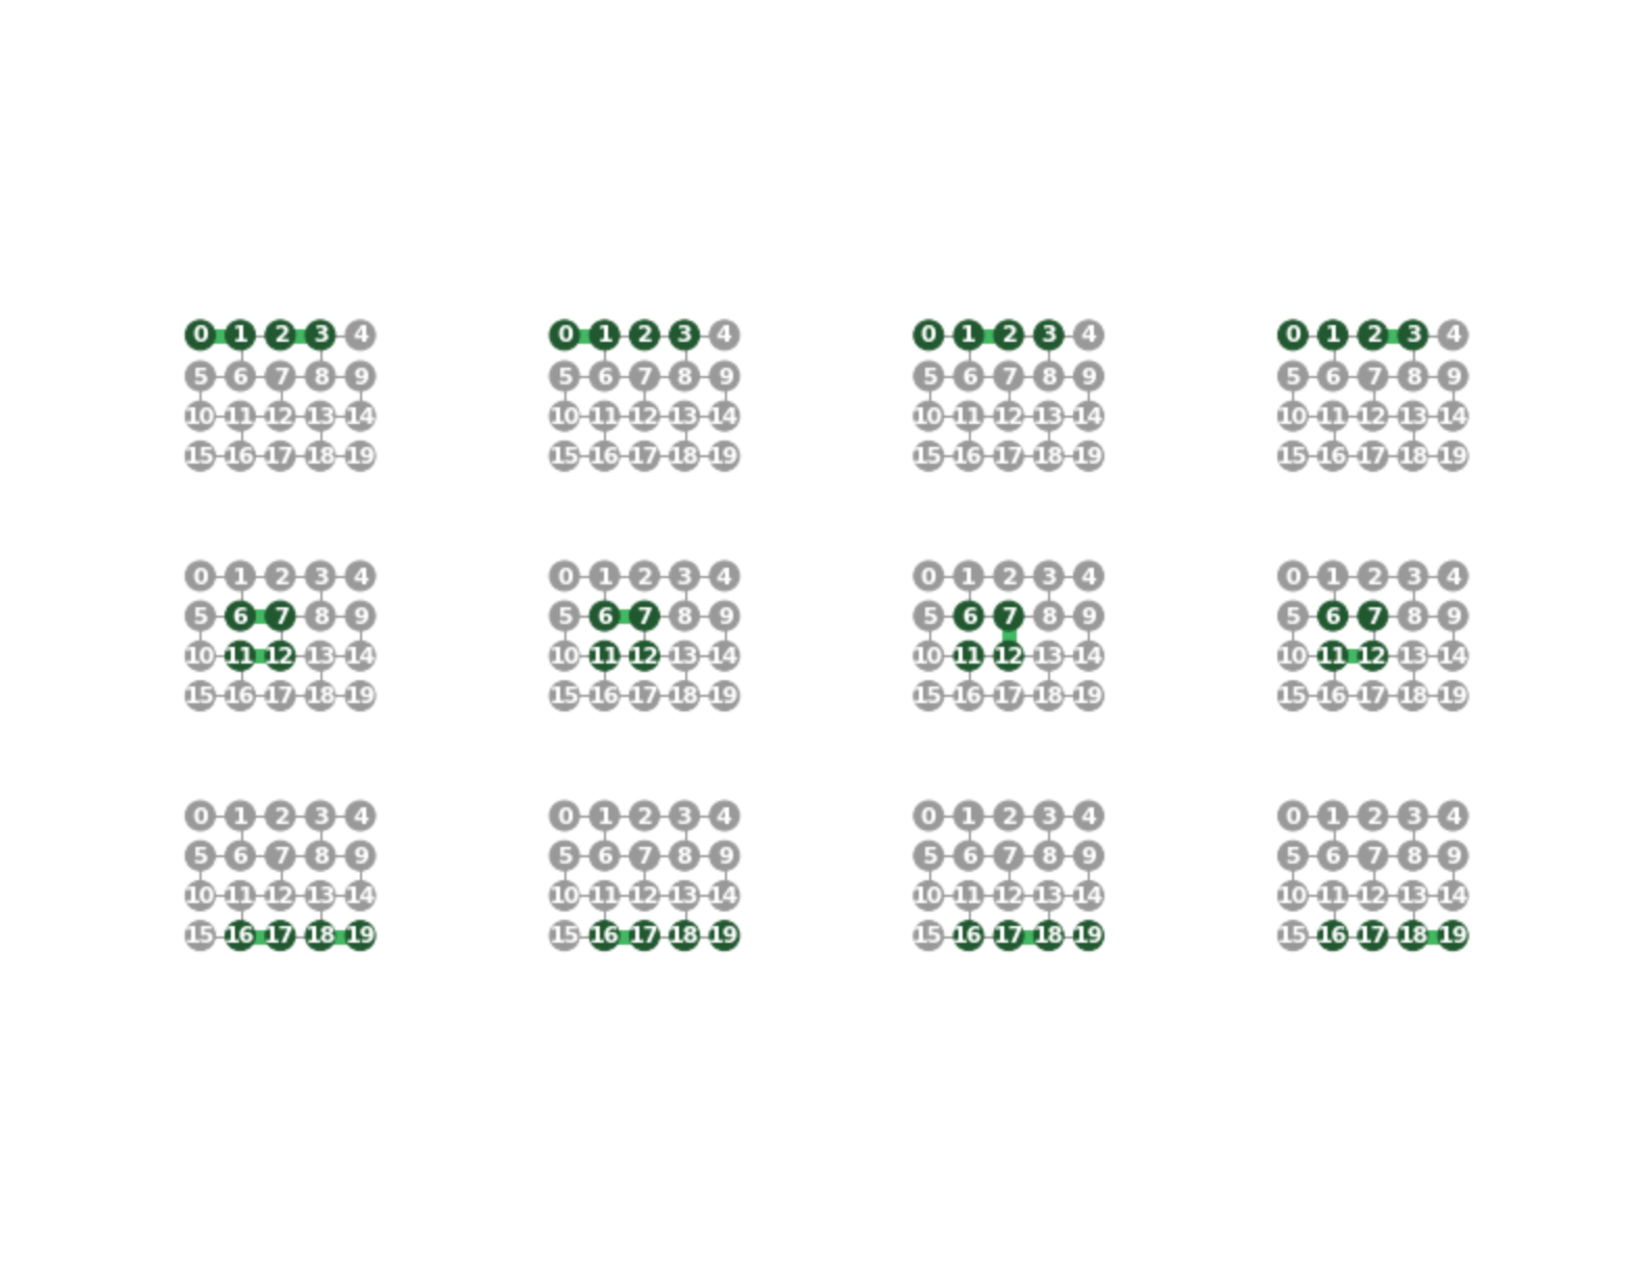
\includegraphics[scale=0.55]{BoeblingenCycles.pdf}
% %    \caption{The CNOT cycles used to calculate the process infidelities on 20-qubit IBM Q Boeblingen device.}
% %    \label{fig:BoeblingenCycles}
% %\end{figure*}

% % The relationship between average process infidelity  and average gate infidelity is
% % \begin{equation}
% % % \label{eq:avg process to gate infidelity conversion}
% %     r\equiv \frac{d-1}{d}(1-p) \label{eq:err_rate}
% % \end{equation}
% % where d is the dimension of the system and p is the randomized benchmarking decay rate~\cite{Qi2019}. 





% \subsection{Calculating Quantum Capacity (QCAP) Bound}
% % In Fig.s~\ref{fig:QCapCirc1}, \ref{fig:QCapCirc2}, \ref{fig:QCapCirc1and2} we present the QCAP bound ($e_{IU}$) values calculated as a function of number of Trotter steps for circuits 1, circuit 2 and circuits 1 and 2 together. The data in Fig.~\ref{fig:QCapCirc1} demonstrates that qubit layout [6, 7, 12, 11] on Boeblingen quantum hardware performs the best for almost all runs and in each day of the experiment for Circuit 1. 
% {\color{red}{KYA: I will embed this section into the section above as well}}.
% We also studied quantum capacity (QCAP) bound of CNOT cycles in the TIM Trotterization quantum circuits as a function of the number of Trotter steps. QCAP bound is able to estimate an upper bound on the total variational distance (TVD) without a full quantum simulation by characterizing the error rate of each cycle in the circuit and combining the results. This upper bound assumes the circuit is being run under randomized compiling (RC). Under RC, each dressed cycle of a circuit will have a stochastic error model whose process fidelity is estimated directly by CB. In this setting, errors accumulate in a circuit in a predictable way: the process fidelity of the circuit is the product of the process fidelity of each cycle. This parameter is estimated as this product, with error bars derived from standard propagation of uncertainty techniques. {\color{red}{KYA: Cite QB website.}} 





% %\begin{figure*}[ht!]
%     % \centering
%     % \includegraphics[width=2.2\columnwidth]{final_plot.pdf}
% %    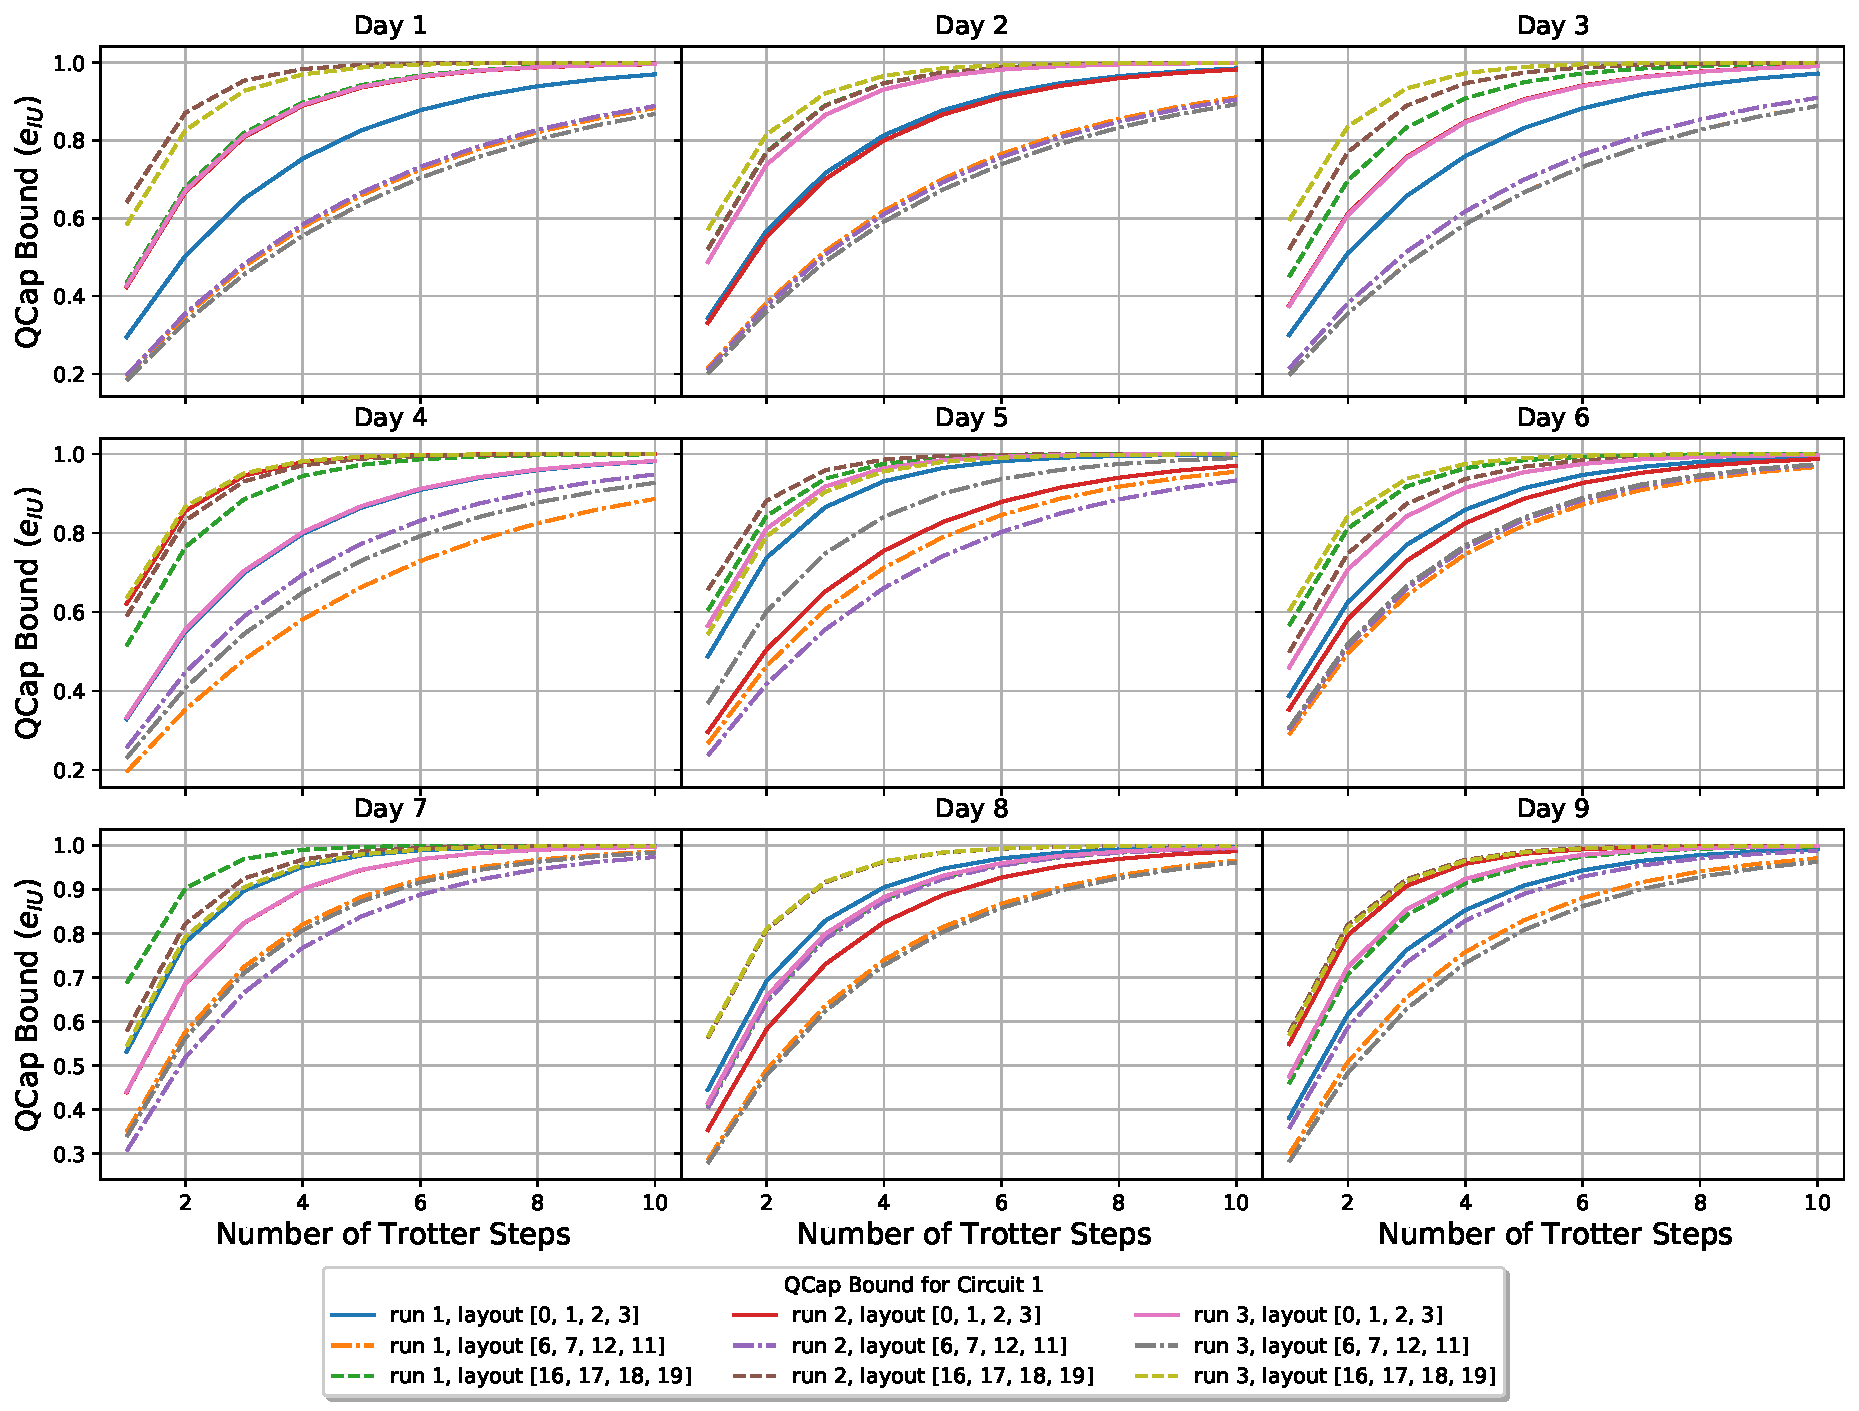
\includegraphics[scale=0.5]{QCapBoundForEachDay_Circ1.pdf}
% %    \caption{QCap bounds calculated using IBM Q Boeblingen hardware as a function of number of Trotter steps for circuit 1, layouts $[0,1,2,3],[6,7,12,11],[16,17,18,19]$, runs 1, 2, and 3 between days 01/23-31/2021 are presented.}
% %    \label{fig:QCapCirc1}
% %\end{figure*}
% %\begin{figure*}[ht!]
%     % \centering
%     % \includegraphics[width=2.2\columnwidth]{final_plot.pdf}
% %    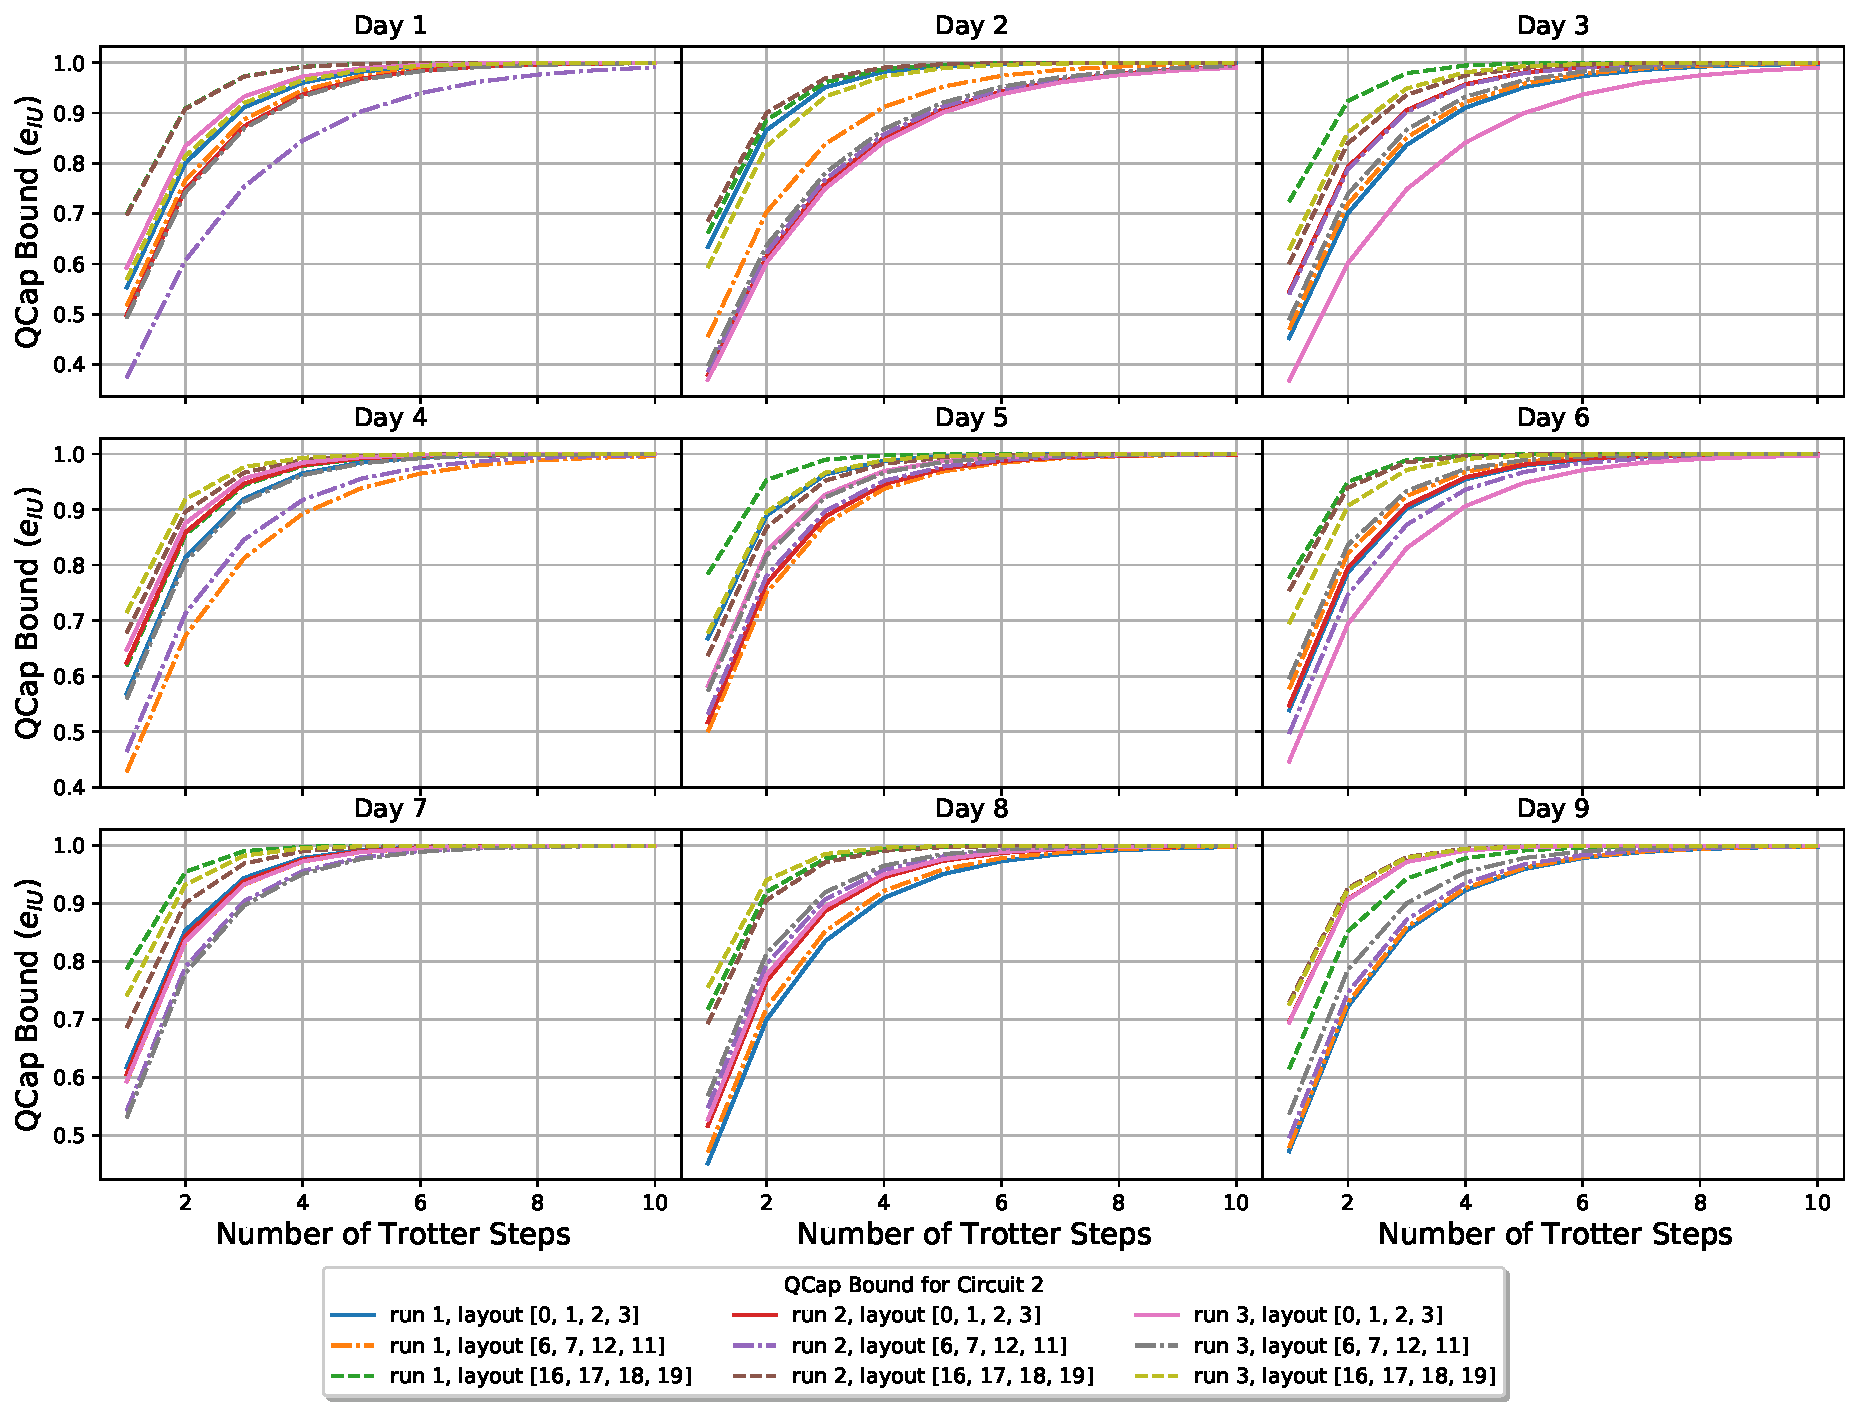
\includegraphics[scale=0.5]{QCapBoundForEachDay_Circ2.pdf}
%  %   \caption{QCap bounds calculated using IBM Q Boeblingen hardware as a function of Trotter steps for circuit 2, layouts $[0,1,2,3],[6,7,12,11],[16,17,18,19]$, runs 1, 2, and 3 between days 01/23-31/2021 are presented.}
% %    \label{fig:QCapCirc2}
% %\end{figure*}

% %\begin{figure*}[ht!]
%     % \centering
%     % \includegraphics[width=2.2\columnwidth]{final_plot.pdf}
% %    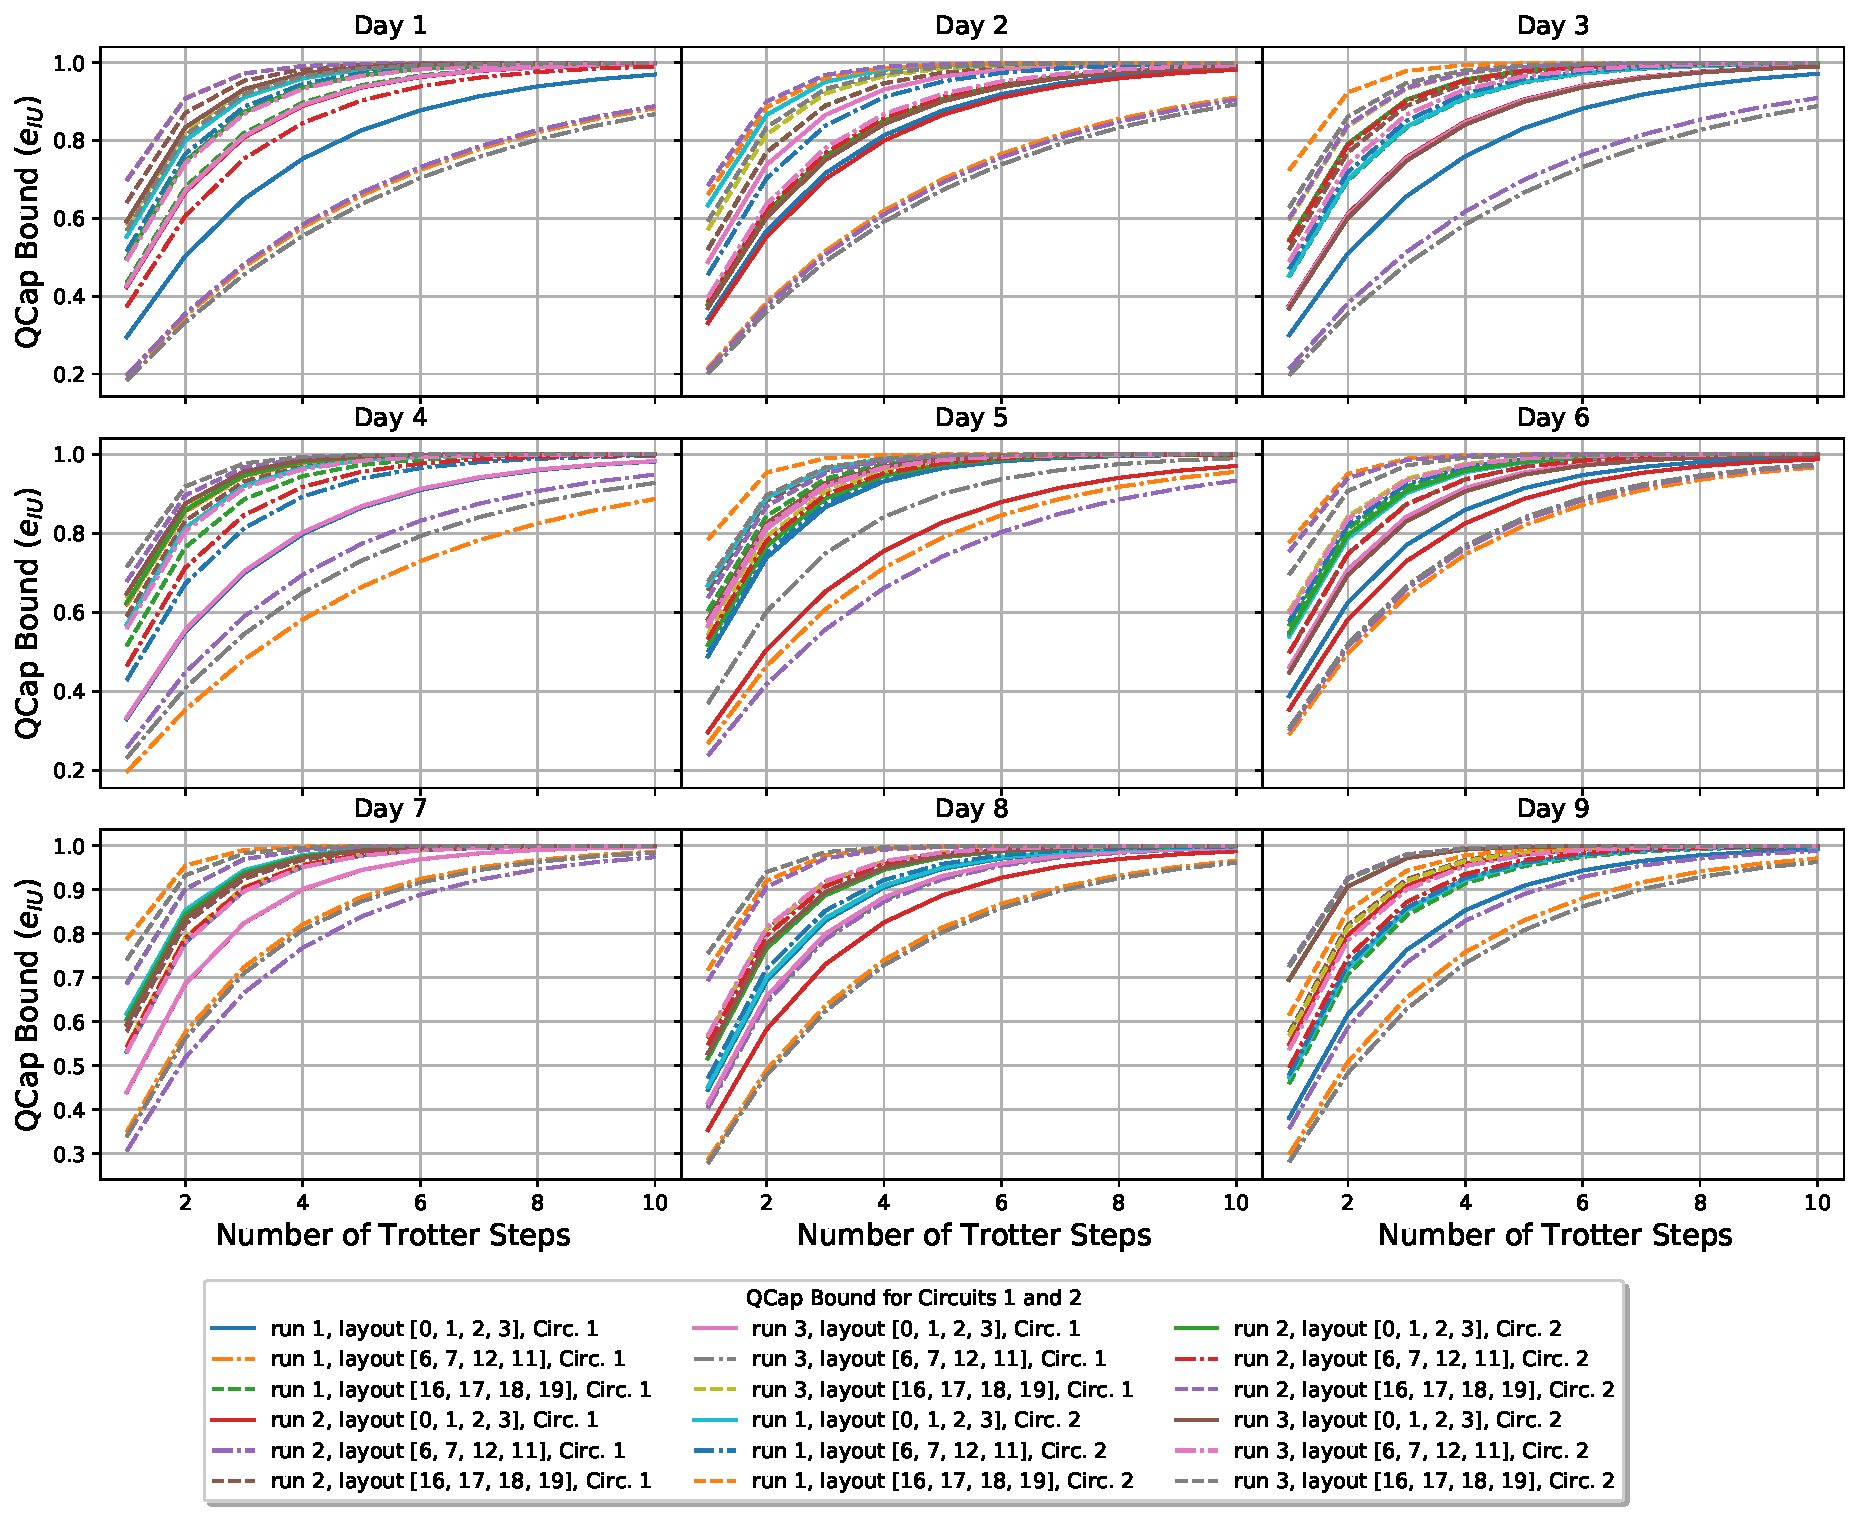
\includegraphics[scale=0.5]{QCapBoundForEachDay_Circ1andCirc2.pdf}
% %    \caption{QCap bounds calculated using IBM Q Boeblingen hardware as a function of number of Trotter steps for circuit 1 and 2 are compared for layouts $[0,1,2,3],[6,7,12,11],[16,17,18,19]$, runs 1, 2, and 3 between days 01/23-31/2021 are presented.}
% %    \label{fig:QCapCirc1and2}
% %\end{figure*}

% The parameters used for QCAP measurements is as follows. Due to limited access to the dedicated mode on Boeblingen device we use sequence lengths of 4 and 16. The number of random circuits in this case is 30 and each of these circuits were run $N_{\text{shots}}=128$. 


% We also computed an estimate to the QCAP bound of CNOT cycles in the TIM Trotterization quantum circuits as a function of the number of Trotter steps calculated from CNOT error rates reported by IBM. To this end, we used the expression for relationship between the average process fidelity and the average gate fidelity as seen in \eqref{eq:err_rate}. For a quantum circuit with $N$ CNOT gates then the QCAP bound calculated using CNOT error rates provided by IBM which are obtained using randomized benchmarking is
% \begin{equation}
%     \text{QCAP}_{\text{RB}}=1-\prod_{i=1}^N\left(1-\frac{d+1}{d} r_i\right)~.\label{eq:QCAP_RB}
% \end{equation}
